\documentclass[a4paper]{article}

%% Language and font encodings
\usepackage[british]{babel}
\usepackage[utf8x]{inputenc}
\usepackage[T1]{fontenc}
\usepackage{float}

%% Sets page size and margins
\usepackage[a4paper,top=3cm,bottom=4cm,left=3cm,right=3cm,marginparwidth=1.75cm]{geometry}

%% Useful packages
\usepackage{amsmath}
\usepackage{graphicx}
\usepackage[framed,numbered,autolinebreaks,useliterate]{mcode}
\usepackage[toc,page]{appendix}
\usepackage{wasysym}
\usepackage[outdir=./]{epstopdf}


\usepackage[parfill]{parskip}

\author{Jacobus Hertzog\\
  \texttt{jjh113@ic.ac.uk}}
\title{Wavelets And Applications Coursework: \\ Sampling Signals with Finite Rate of Innovation with an Application to Image Super Resolution}
\date{\today}



\begin{document}
\maketitle

\tableofcontents
\newpage


\section{Strang-Fix Conditions}
\subsection{Exercise 1}

In this exercise, we show that a function satisfying the Strang-Fix conditions with N+1 moments is able to reproduce polynomials of any order up to N. The Strang-Fix conditions are important as any function satisfying them is a valid member of the polynomial reproducing kernel family. Daubechies scaling functions are an example of functions that satisfy the Strang-Fix conditions and are thus members of this family. As a result if we wish to reproduce polynomials of order 0-3 with a Daubechies scaling function then we require a Daubechies filter with $N+1=4$ vanishing moments. Therefore we use the scaling function named ’dB4’, shown in figure \ref{fig:ex1_db4}.

Initially $32-L$ coefficients were used, as directed in the coursework specification. L is the support, the range of values for which the scaling function is non-zero. For Daubechies wavelets, the support width is given by $2N-1$, so for 'dB4', the support is 7. This produced 26 coefficients.However, it was discovered that the error of the reconstruction could be reduced when using 32 coefficients. Therefore, 32 coefficients were calculated and used for the remainder of the project.

\begin{figure}[!ht]
    \centering
    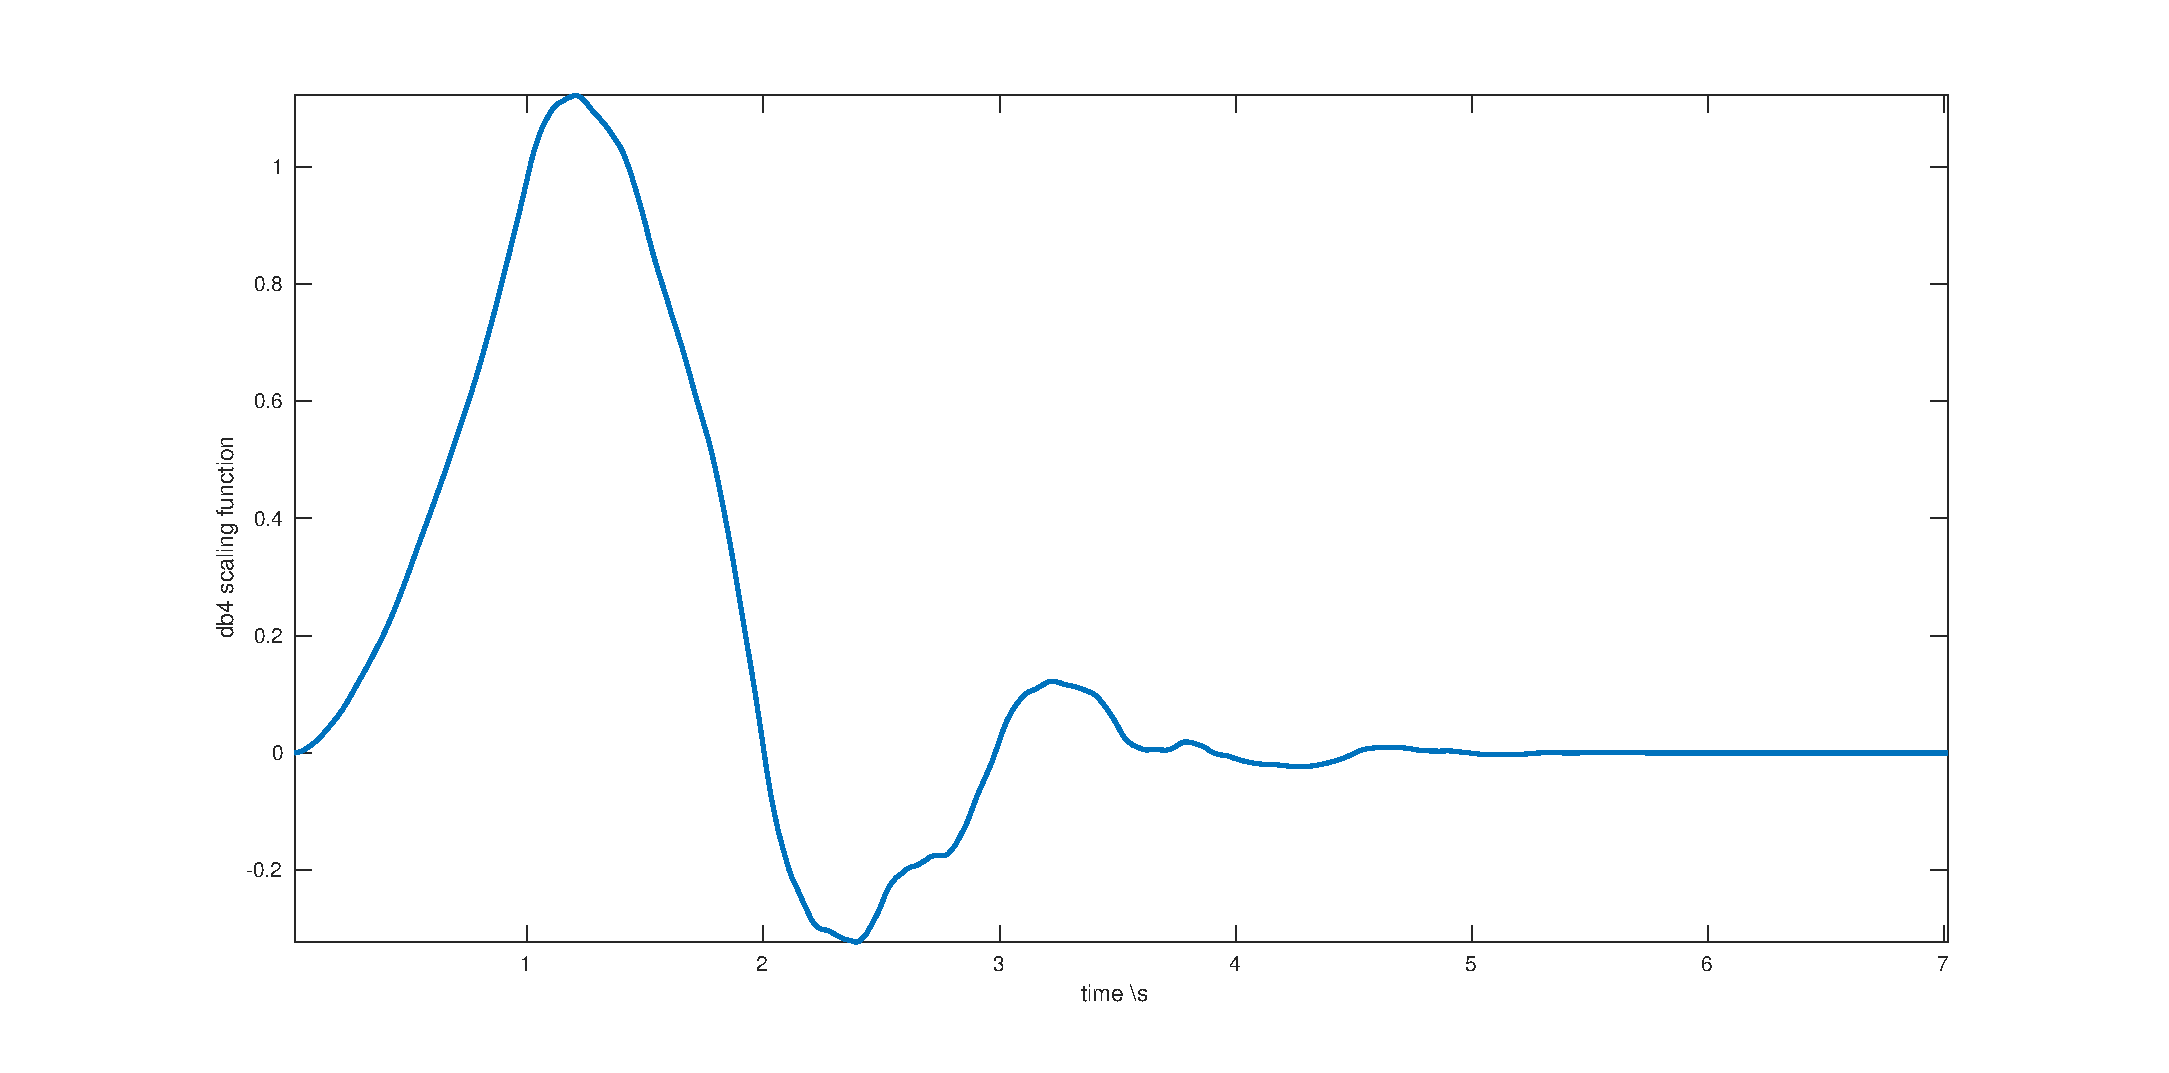
\includegraphics[width=0.5\textwidth]{../images/ex1_db4}
    \caption{dB4 Scaling Function}
    \label{fig:ex1_db4}
\end{figure}

As Daubechies wavelets are orthogonal, so there is no need to calculate the dual basis of the signal in order to find the reconstruction coefficients. The coefficients were instead given by the formula $c_{m,n} = <t^m,\varphi(t/T-n)>$. Once the coefficients are computed, and divided by 64 to account for the sampling rate, they can be multiplied with the appropriate shifted sampling kernel in order to reproduce any piecewise polynomial up to the order given by N.

\begin{figure}[H]
    \centering
    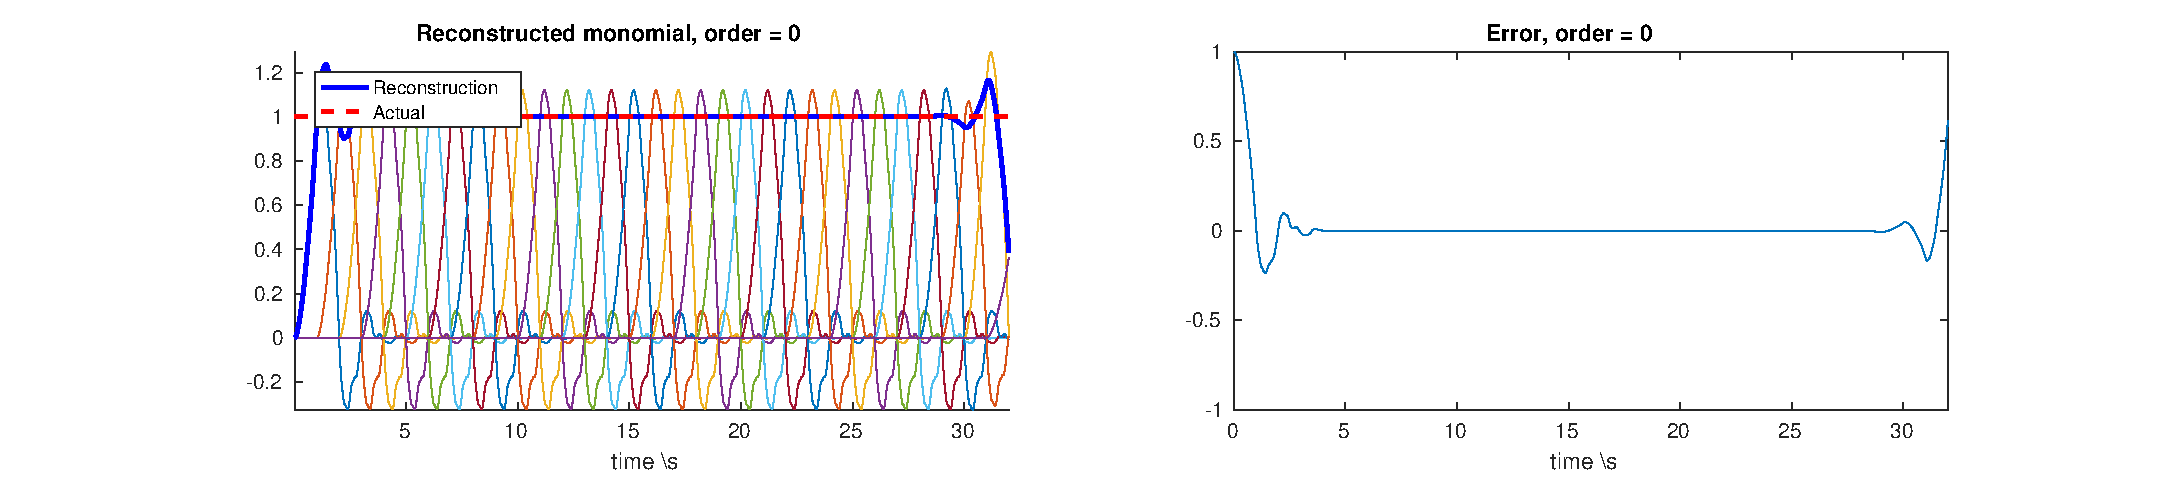
\includegraphics[width=\textwidth]{../images/ex1_0}
    \caption{Reconstruction of 0 order monomial}
    \label{fig:ex1_0}
\end{figure}

\begin{figure}[H]
    \centering
    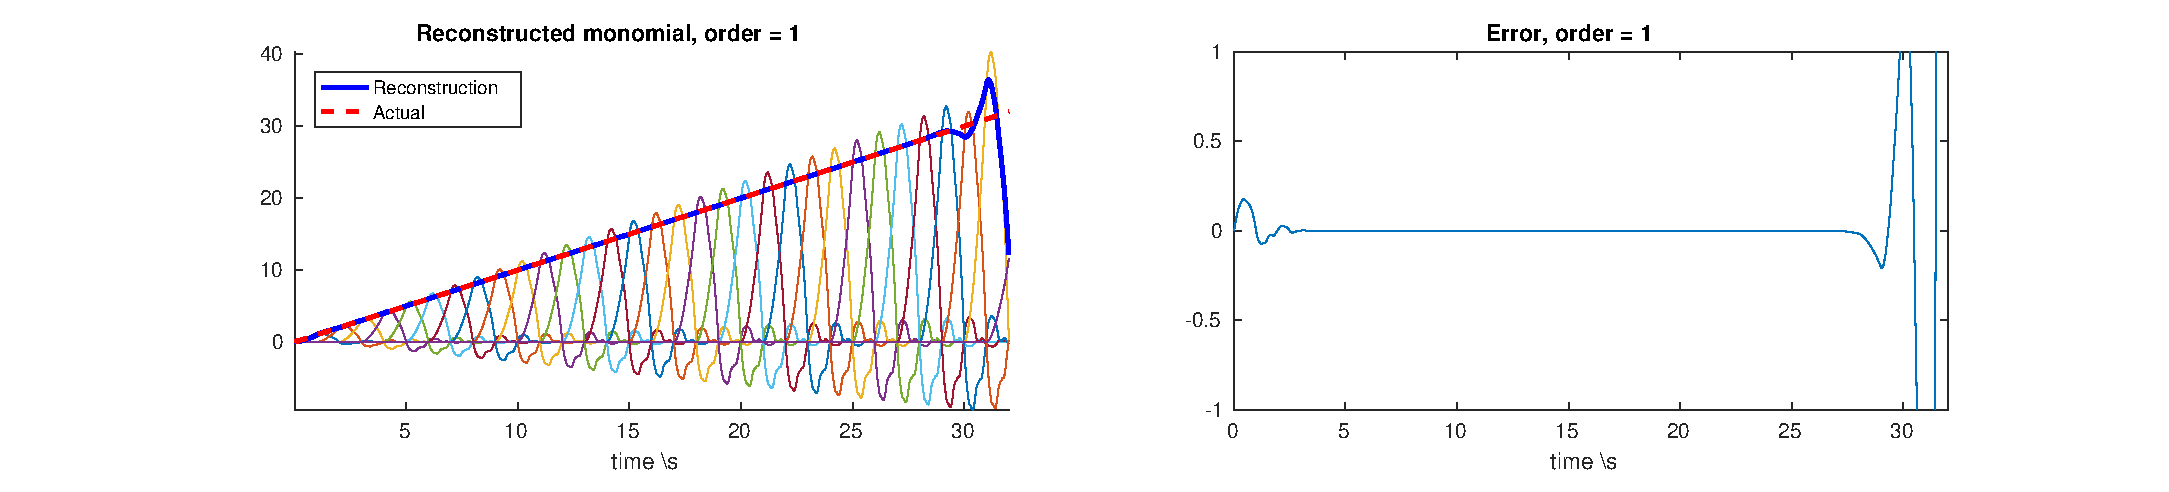
\includegraphics[width=\textwidth]{../images/ex1_1}
    \caption{Reconstruction of 1 order monomial}
    \label{fig:ex1_1}
\end{figure}

\begin{figure}[H]
    \centering
    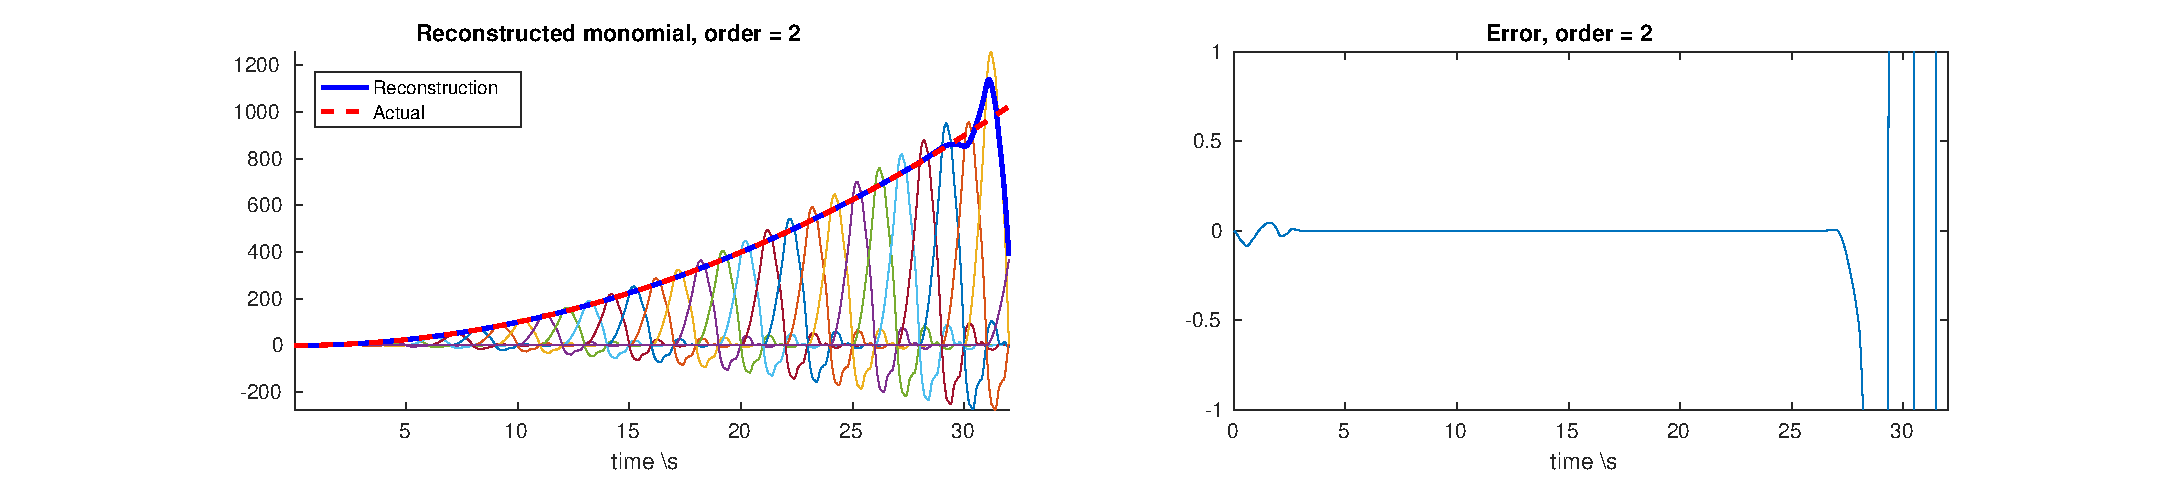
\includegraphics[width=\textwidth]{../images/ex1_2}
    \caption{Reconstruction of 2 order monomial}
    \label{fig:ex1_2}
\end{figure}

\begin{figure}[H]
    \centering
    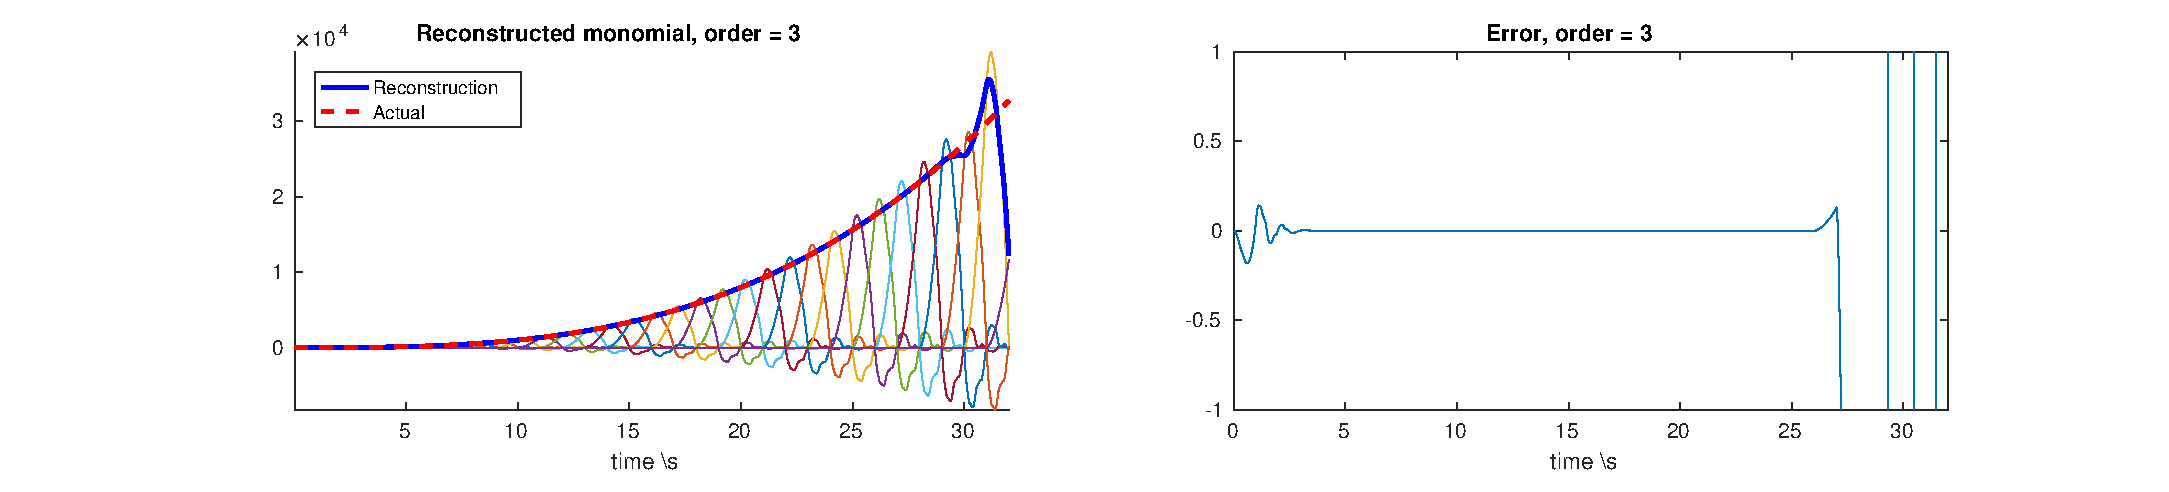
\includegraphics[width=\textwidth]{../images/ex1_3}
    \caption{Reconstruction of 3 order monomial}
    \label{fig:ex1_3}
\end{figure}

The plots in figures \ref{fig:ex1_0},\ref{fig:ex1_1}, \ref{fig:ex1_2}, and \ref{fig:ex1_3} show that the sampling kernel is able to reproduce the polynomials perfectly, excluding the edges of the reconstruction where the reconstruction has no preceding/following samples to carry on the reconstruction. However, when we attempt to reconstruct a polynomial of order 4, as shown in figure \ref{fig:ex1_4}, errors are introduced. 

\begin{figure}[H]
    \centering
    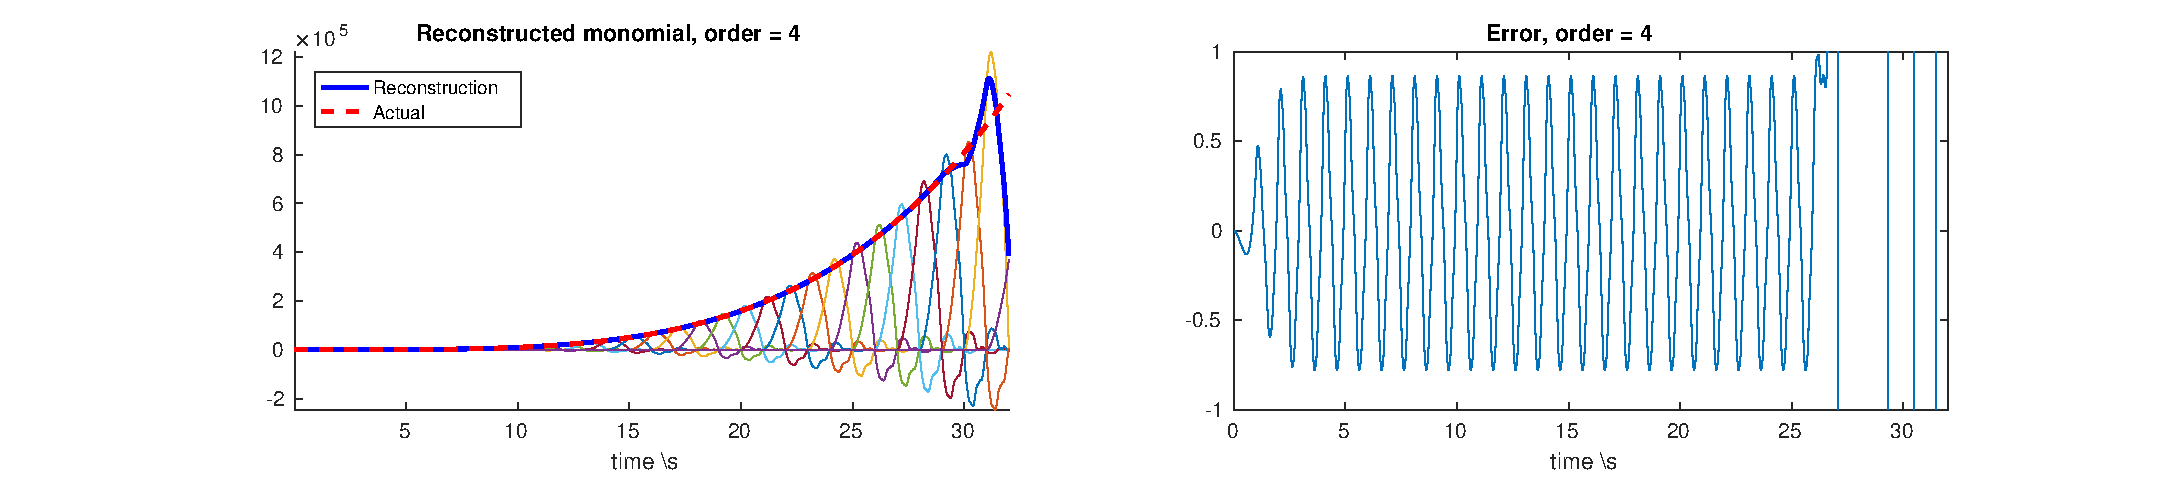
\includegraphics[width=1\textwidth]{../images/ex1_4}
    \caption{Attempted reconstruction of 4 order monomial}
    \label{fig:ex1_4}
\end{figure}


\subsection{Exercise 2}

The next exercise was similar, but a bit more complex. Rather than using a Daubechies scaling function, a B-Spline was used. B-Splines are produced by iteratively convolving a rectangular function, or Haar wavelet. In order to reproduce polynomials of order 0-3, a B-Spline of order 3, $\beta_3$, was produced by convolving the Haar wavelet four times. The result is shown in figure \ref{fig:ex2_1}

\begin{figure}[H]
    \centering
    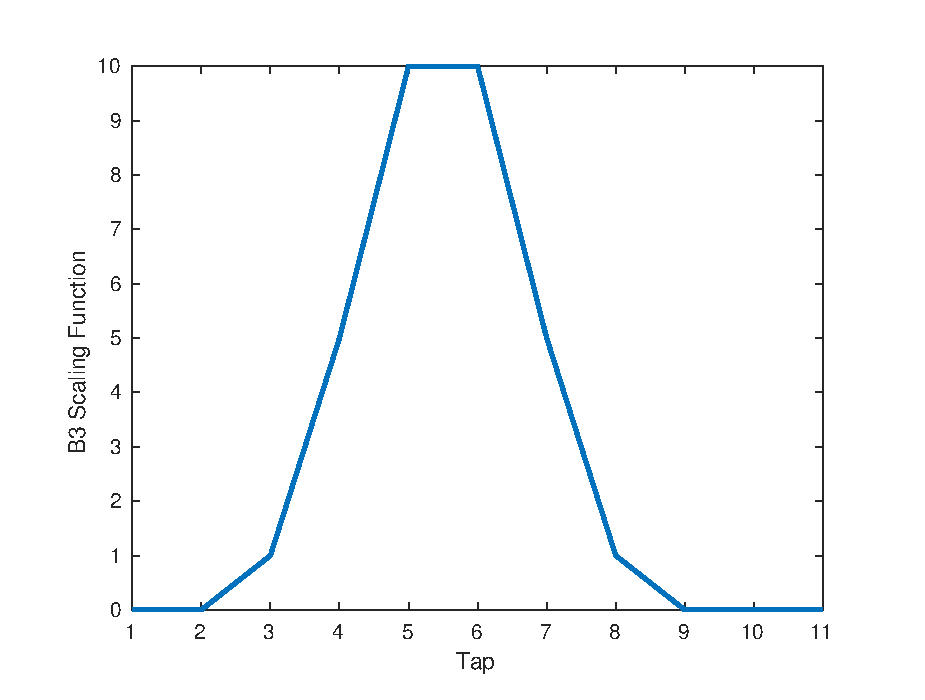
\includegraphics[width=0.5\textwidth]{../images/ex2}
    \caption{$\beta_3$ Scaling Function}
    \label{fig:ex2_1}
\end{figure}

With the exception of $\beta_0$, which is equivalent to the Haar wavelet, B-Splines are not orthogonal, and as a result, it is necessary to calculate the dual basis of $\beta_3$ in order to find the coefficients for the polynomial reproduction. Unfortunately, I was not able to compute the dual basis of $\beta_3$ and was therefore unable to complete the rest of the exercise.

\section{The Annihilating Filter Method}
\subsection{Exercise 3}

This exercise involved writing a program that would find the annihilating filter of a signal $\tau[m]$. This was a straightforward case of following the instructions given. Given that $h[1] = 1$, the annihilating filter was found by solving equation \ref{eq:ex3_1}:

\begin{equation}
\begin{pmatrix}
h[1] \\
h[2] \\
\vdots \\
h[K]
\end{pmatrix}
=
\begin{bmatrix}
\tau[K-1] & \tau[K-2] & \dotsb & \tau[0] \\
\tau[K-1] & \tau[K-1] & \dotsb & \tau[1] \\
\vdots & \vdots & \ddots & \vdots \\
\tau[N-1] & \tau[N-2] & \dotsb & \tau[N-K]
\end{bmatrix}^{-1}
-\begin{pmatrix}
\tau[K] \\
\tau[K+1] \\
\vdots \\
\tau[N]
\end{pmatrix}
\end{equation}
\label{eq:ex3_1}

Once the annihilating filter was found, the locations of the Diracs, $t_k$, could be easily found by finding the roots of h. Next, the Vandermonde system in equation \ref{eq:ex3_2} was solved to find the weights, $a_k$.

\begin{equation}
\begin{pmatrix}
a_0 \\
a_1 \\
\vdots \\
a_{K-1}
\end{pmatrix}
=
\begin{bmatrix}
1 & 1 & \dotsb & 1 \\
t_0 & t_1 & \dotsb & t_{K-1} \\
\vdots & \vdots & \ddots & \vdots \\
t^{K-1}_{0} & t^{K-1}_{1} & \dotsb & t^{K-1}_{K-1}
\end{bmatrix}^{-1}
\begin{pmatrix}
\tau[0] \\
\tau[1] \\
\vdots \\
\tau[K-1]
\end{pmatrix}
\end{equation}
\label{eq:ex3_2}

This algorithm was applied to the $\tau$ variable obtained from\texttt{tau.mat}, the file provided to us. The annihilating filter $h[n]$ value are shown in table \ref{tab:ex3_1} and the recovered locations and weights are shown in table \ref{tab:ex3_2}. The reconstructed stream of Diracs is shown in figure \ref{fig:ex3_1}.

\begin{table}[H]
    \parbox{.45\linewidth}{
    \centering
    \begin{tabular}{|c|c|c|}
        \hline
        $h[0]$     & $h[1]$     & $h[2]$ \\ \hline
        1.0000       & -29.6250  & 219.0937\\ \hline
    \end{tabular}
    \caption{The annihilating filter coefficients.}
    \label{tab:ex3_1}
    }
    \hfill
    \parbox{.45\linewidth}{
    \centering
    \begin{tabular}{|c|c|c|}
        \hline
        $k$     & $t_k$     & $a_k$ \\ \hline
        0       & 15.3750   & 0.7800\\ \hline
        1       & 14.2500   & 1.3200\\ \hline
    \end{tabular}
    \caption{Results of the annihilating filter applied to \texttt{tau.mat}.}
    \label{tab:ex3_2}
    }
\end{table}

\begin{figure}[H]
    \centering
    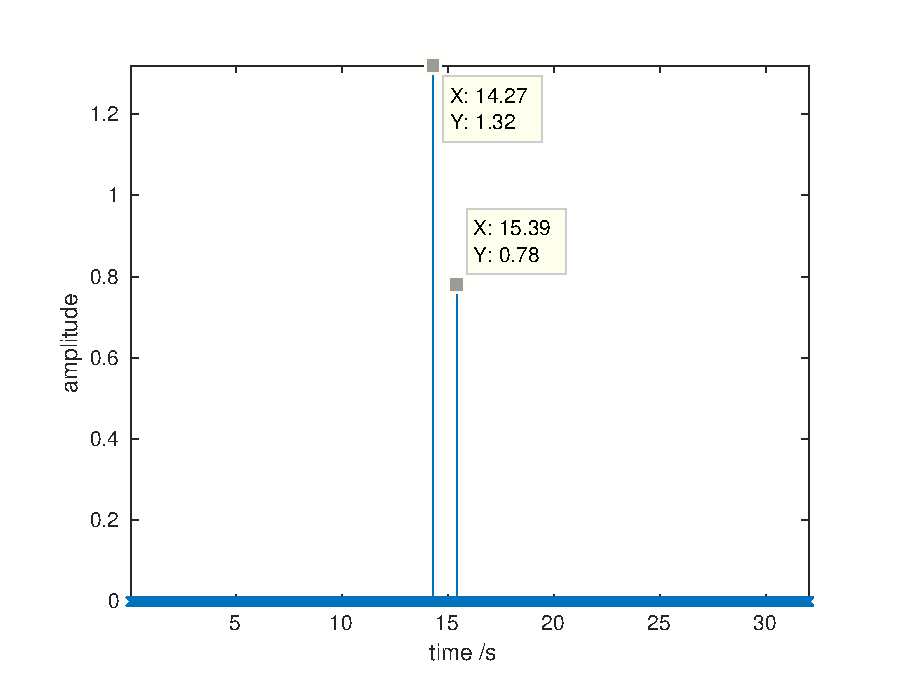
\includegraphics[width=0.5\textwidth]{../images/ex3}
    \caption{Reconstruction of Dirac Stream}
    \label{fig:ex3_1}
\end{figure}

To verify that the annihilating filter is correctly constructed, we can perform a simple test. By definition, the convolution of the annihilating filter $h$ with the  $\tau$ should result in a zero output at the centre. The result of the convolution $y = h*\tau$, is shown in \ref{tab:ex3_3}. The only important results here are those at index 2 and 3, as the other values are cases where the convolution cannot shift the signals fully through one another. Since these are both zero

\begin{table}[H]
    \centering
    \begin{tabular}{|c|c|c|c|c|c|}
        \hline
		$y[0]$ & $y[1]$ & $y[2]$ & $y[3]$ & $y[4]$ & $y[5]$ \\ \hline
		2.10 & -31.40 & 0 & 0 & -98016.19 & 1457963.78 \\ \hline

    \end{tabular}
    \caption{Results of the convolution $y = h*\tau$}
    \label{tab:ex3_3}
\end{table}

Since this method was to be reused  for other exercises, it was developed into a function called \mcode{annihilatingFilterMethod.m}


\section{Sampling Diracs}
\subsection{Exercise 4}

This exercise required us to construct our own Dirac stream, sample it with a sampling kernel, and perform the annihilating filter method to reconstruct the signal from the samples. The first step in this process was selecting parameters for the Dirac stream. The Dirac stream is given by the equation $x(t) = \sum^{K-1}_{k=0} a_k\delta(t-t_k)$,  so when $K$ = 2, we have a stream with two Diracs and we need to select two values for location and weight. These are given in the table \ref{tab:ex4_1}.

\begin{table}[H]
    \parbox{.45\linewidth}{
    \centering
    \begin{tabular}{|c|c|c|}
        \hline
        $k$     & $t_k$     & $a_k$ \\ \hline
        0       & 12.5   & 5\\ \hline
        1       & 23.0   & 2\\ \hline
    \end{tabular}
    \caption{Original weights and locations of $x(t)$}
    \label{tab:ex4_1}
    }
    \hfill
    \parbox{.45\linewidth}{
    \centering
    \begin{tabular}{|c|c|c|}
        \hline
        $k$     & $t_k$     & $a_k$ \\ \hline
         0       & 12.5   & 5\\ \hline
        1       & 23.0   & 2\\ \hline
    \end{tabular}
    \caption{Retrieved weights and locations from the annihilating filter method}
    \label{tab:ex4_2}
    }
\end{table}


The signal was sampled using the same 'dB4' scaling function as shown in figure \ref{fig:ex1_db4} from exercise 1. This is because we know that the sampling kernel $\varphi(t)$ must be able to reproduce polynomials of order $N \geq 2K-1$, so for $K=2$, $N\geq 3$.

The next step in the process was to sample the signal. The samples were produced using the formula $y_n = <x(t),\varphi(t/T-n)>$. Once these samples had been computed, the moments of the signal were calculated as the product of the samples and the sampling kernel's coefficients. Since the same scaling function is used as in exercise 1, the coefficients were simply reused. The sequence of moments was thus given by the formula $\tau(m)=\sum_nc_{m,n}y[n]$.

Now that the sequence of moments had been found, the signal was recovered using the annihilating filter function \mcode{TODO anni}, developed in exercise 3. The retrieved locations and weights are shown in \ref{tab:ex4_2} results of the reconstruction are shown in figure \ref{fig:ex4_1}. It can be clearly seen that the reconstruction fully matches the original signal.


\begin{figure}[H]
    \centering
    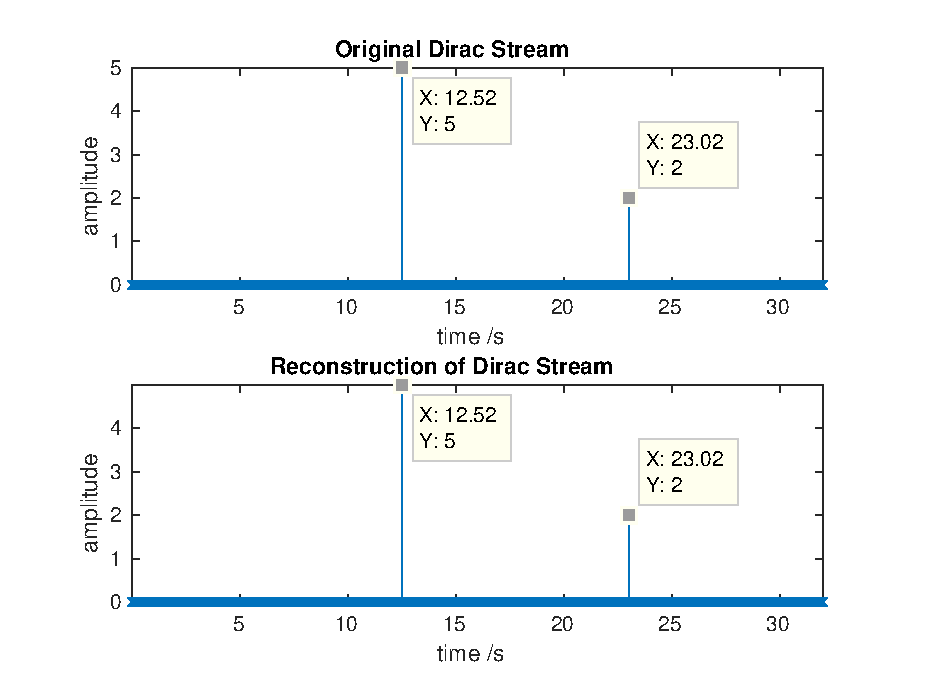
\includegraphics[width=\textwidth]{../images/ex4}
    \caption{Original Signal and Reconstruction}
    \label{fig:ex4_1}
\end{figure}

\subsection{Exercise 5}

In this exercise, the signal samples from an unknown signal were provided in the file \texttt{sample.mat}. By applying the same method as in exercise 4, this signal could be reconstructed. As described previously, the moments were computed using the formula $\tau(m)=\sum_nc_{m,n}y[n]$, and the annihilating filter method was applied. The results of the reconstruction are shown in table \ref{tab:ex5_1} and figure \ref{fig:ex5_1}.

\begin{table}[H]
    \centering
    \begin{tabular}{|c|c|c|}
        \hline
        $k$     & $t_k$     & $a_k$ \\ \hline
		0 & 14.3750 & 2.6300\\ \hline
        1 & 17.5000 & 1.4800 \\ \hline
    \end{tabular}
    \caption{The location and weights of the Diracs from the unknown signal.}
    \label{tab:ex5_1}
\end{table}

This result can be verified by taking samples of the reconstructed signal and checking whether this matches the original set of samples. Using the 'db4' scaling function and the formula $y_n = <x(t),\varphi(t/T-n)>$ from the previous exercise, the samples were calculated and are shown in \ref{fig:ex5_1} alongside the original samples. The two waveforms are identical, verifying that the reconstructed signal is correct.

\begin{figure}[H]
    \centering
    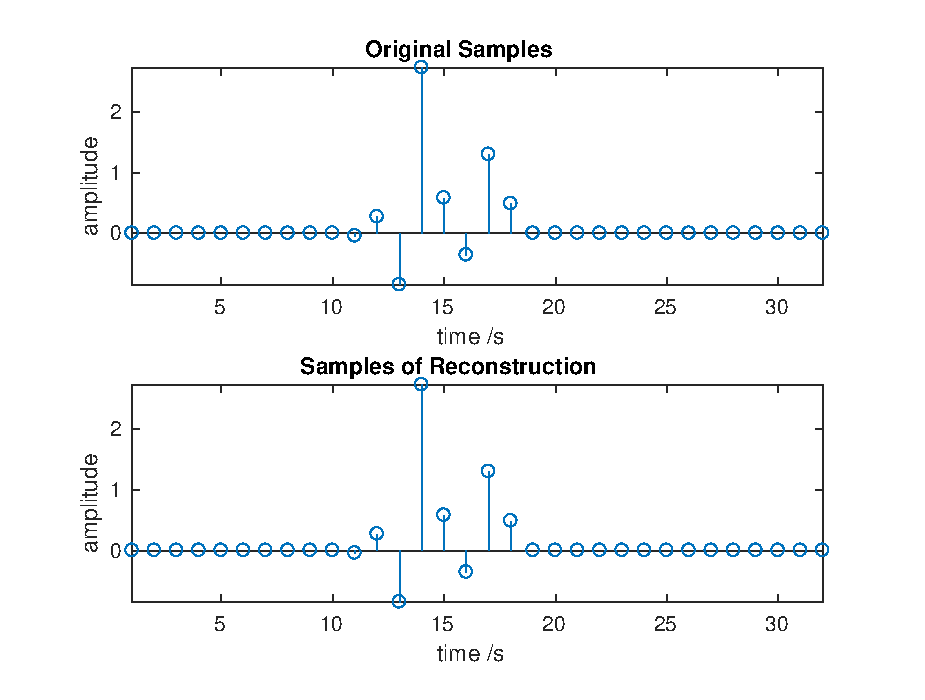
\includegraphics[width=\textwidth]{../images/ex5_2}
    \caption{Original Signal and Reconstruction}
    \label{fig:ex5_1}
\end{figure}


\section{Reconstruction in the Presence of Noise}
\subsection{Exercise 6}

This exercise simply involved calculating generating a Dirac stream and finding the moments as previously done, and then adding Gaussian noise to the moments. This also needs to be done for different values of $N$ and variances, $\sigma^2$ of the Gaussian noise. 

In order to make this process easier, a function named \mcode{generateMoments} was written that would take in a Dirac stream and the desired N value, generate the appropriate Daubechies scaling function 'dBN', generate the polynomials $t^m$, obtain the coefficients, sample the signal and finally combine the coefficients and the samples to procude the moments of the signal. We are given that $N > 2K$. Note that because noise is added, $N = 2K$ is no longer viable as it has been in previous exercises. $K=2$, so $N >4$. The range $N = [5:8]$ was chosen for testing.

After each sequence of moments was generated, noise was added to it. The noise values were generated simply using the \mcode{randn} to generate normally distributed values. Multiplying these values by the standard deviation, $\sigma$, produced the noise values that were added to the moments. The range of moments selected was $\sigma^2 \in {0.001, 0.01, 0.1, 1, 10}$. An example of a sampling kernel and noisy moment signal are shown in figure \ref{fig:ex6_1}.


\begin{figure}[H]
    \centering
    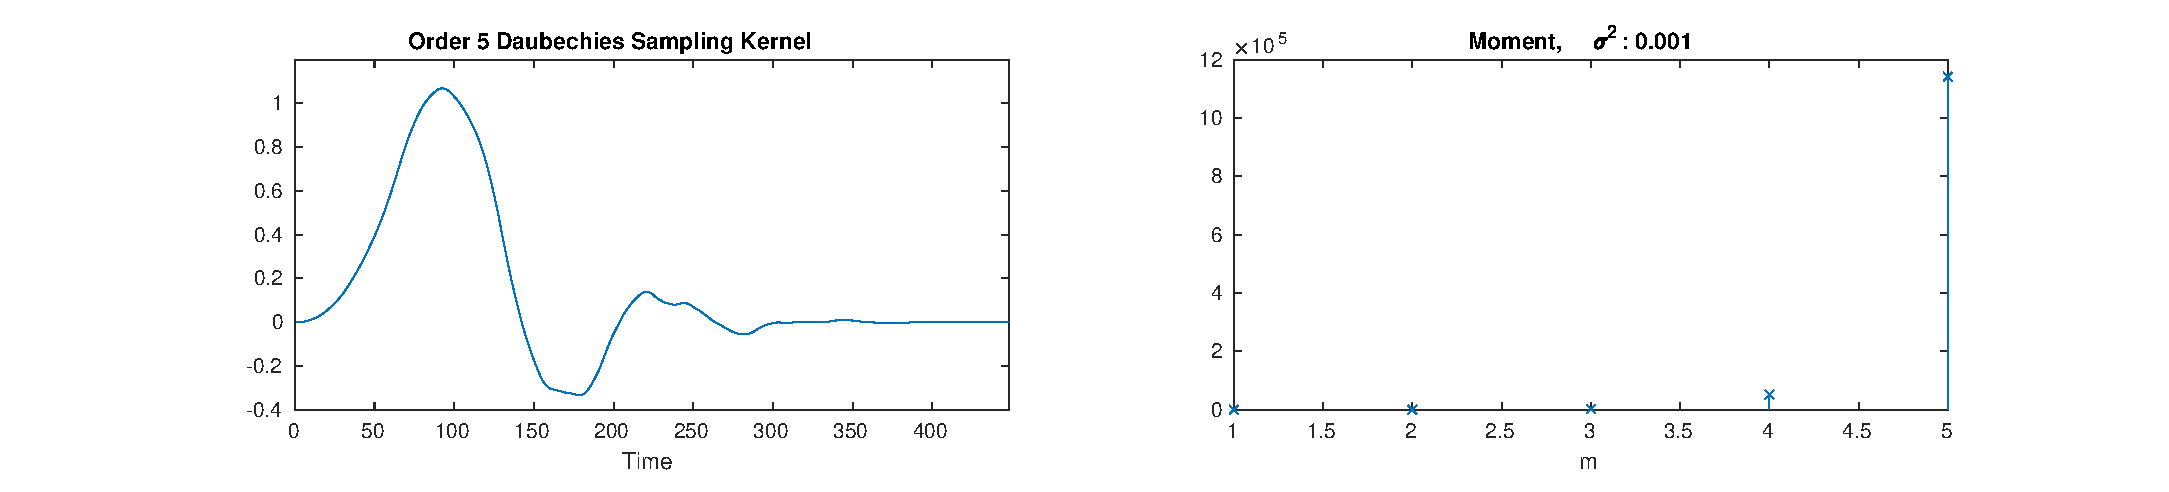
\includegraphics[width=\textwidth]{../images/ex6}
    \caption{Sampling Kernel and Moments Signal with Noise Added}
    \label{fig:ex6_1}
\end{figure}


\subsection{Exercise 7}

In this exercise, the reconstruction of the signals from noisy moments was attempted. This could be done using the standard annihilating filter seen in previous exercises, but only with limited success. It can be improved upon using the Total Least-Squares (TLS) approach. This involves computing the annihilating filter using Singular Vector Decomposition(SVD). A Toeplitz matrix $S$ is broken down into $S = U\Lambda V^T$. The final column of $V$ is then taken to be the annihilating filter $h[n]$. Once this is complete, the locations $t_k$ and the weights $a_k$ are found in the standard way.

Beyond this, the results can be further improved by performing the Cadzow routine upon the Toeplitz matrix $S$. The SVD is taken again, producing $S = U\Lambda V^T$, and then the $\Lambda$ matrix is modified. This is a diagonal matrix containing the eigenvalues of S, and all but the $K$ largest eigenvalues are set to zero to produce $\Lambda'$. These values set to zero are components of the noise, so by setting them to zero, the matrix is being 'denoised'. Then $S'$ is reformed as $S' = U\Lambda'V^T$, and the process may be repeated to reduce the noise further, or the LTS method can be performed to find estimates of the Dirac stream.

The normal annihilation method was able to detect two Diracs in the stream, but there were heavy errors present in the estimations of location and weight that grew larger as the noise increased. This is expected, as errors introduced to the values of the moments will naturally throw off the estimations. There was no observable variation with different values of $N$.

When TLS was introduced, it was more resistant to noise until $\sigma^2 = 10$ when the system could no longer detect two Diracs. Cadzow improved the system even further, allowing detection more accurately at higher noise levels. Unfortunately I have run out of time and am not able to include these figures in the report.

\appendix
\section{Ex1}
\lstinputlisting{../ex1_daubechies.m}

\section{Ex2}
\lstinputlisting{../ex2_Bspline.m}

\section{Ex3}
\lstinputlisting{../ex3_annihilating_filter.m}

\section{annihilatingFilterMethod.m}
\lstinputlisting{../annihilatingFilterMethod.m}

\section{Ex4}
\lstinputlisting{../ex4_sampling_diracs.m}

\section{Ex5}
\lstinputlisting{../ex5_sampling_diracs.m}

\section{Ex6}
\lstinputlisting{../ex6_noisy_signal.m}

\section{momentsGenerator.m}
\lstinputlisting{../momentsGenerator.m}

\section{Ex7 with No Enhancements}
\lstinputlisting{../ex7_none.m}

\section{Ex7 with LTS}
\lstinputlisting{../ex7_tls.m}

\section{annihilatingFilterMethodTLS.m}
\lstinputlisting{../annihilatingFilterMethodTLS.m}

\section{Ex7 with LTS and Cadzow}
\lstinputlisting{../ex7_cadzow.m}

\section{annihilatingFilterMethodCadzow.m}
\lstinputlisting{../annihilatingFilterMethodCadzow.m}

\end{document}
